\chapter{Subregion-subalgebra duality}

Chapters 2--6 built the tools for the idea of this chapter. The claim is simple to state, and its
consequences are large: \textbf{in the strict large-$N$ limit, an arbitrary bulk spacetime region is not
merely \emph{related to} a boundary operator subalgebra; it \emph{is} one.} This is not an approximation,
and there is no correction term to add at this order. The algebra of the bulk region and the boundary
algebra are the same mathematical object, described in two different languages.

\section{General formulation}

\subsection*{Where the identification comes from}

Chapter 6 identified two Hilbert spaces. The first is the bulk Fock space. It is built by ordinary
quantization of small fluctuations around a classical background. The second is the boundary GNS Hilbert
space. It is built, through the GNS construction, from the algebra of boundary operators that survive the
large-$N$ limit. Since these are the same Hilbert space, the algebras of all bounded operators on them are
also the same:
\begin{equation}
B(\HH_\Psi^{\text{Fock}}) = B(\HH_\Psi^{\text{GNS}}) .
\label{eq:full_algebra_identity}
\end{equation}
This equation hides a small surprise. $B(\HH_\Psi^{\text{Fock}})$ is naturally built from data on a single
bulk Cauchy slice, because canonical quantization only needs one moment of time. $B(\HH_\Psi^{\text{GNS}})$
is built from operators on the entire boundary spacetime, or, by the time-band result of Chapter 6, at least
on a finite time band. These look like objects of different sizes. They are reconciled by the fact that the
bulk has one more spatial dimension than the boundary. The data of this extra dimension, spread over one
bulk Cauchy slice, is matched by a stretch of boundary \emph{time}, not boundary space. This is a first hint
of a general phenomenon that Chapter 8 develops in full: boundary time and bulk radial position are closely
linked.

At the free (quadratic) level, different bulk fields do not interact. So both the Hilbert space and its
operator algebra split into independent tensor factors, one for each field species $i$:
$\HH_\Psi^{\text{GNS}}=\bigotimes_i\HH_{\Psi,i}^{\text{GNS}}$, with $\HH_{\Psi,i}^{\text{Fock}}=
\HH_{\Psi,i}^{\text{GNS}}$ for each field separately. Nothing conceptually new happens here. It is
bookkeeping: the identification holds field by field, not just for the whole theory at once.

\subsection*{The duality, stated precisely}

Equation \eqref{eq:full_algebra_identity} is an identity between entire operator algebras. So it must also
hold subalgebra by subalgebra. Take any open bulk subregion $b$ of a Cauchy slice. It has a bulk operator
algebra $\widetilde\M_b \subset B(\HH_\Psi^{\text{Fock}})$. (Throughout this chapter, bulk algebras carry a
tilde, to keep them visually distinct from boundary algebras.) By \eqref{eq:full_algebra_identity}, this is
also a subalgebra of $B(\HH_\Psi^{\text{GNS}})$. When we view it as a boundary algebra we call it $\M_b$:
\begin{equation}
\widetilde\M_b = \M_b .
\label{eq:subregion_subalgebra}
\end{equation}
Read this as a literal equality, not as an analogy or a matching of some properties. There is one algebra,
with two descriptions.

Chapter 4 explained how an algebra, together with a state, encodes causal structure, entanglement, and
modular flow. Since $\M_b=\widetilde\M_b$, \textbf{the boundary algebra $\M_b$ already encodes the
corresponding structure of the bulk region $b$}. For example, the modular operator of $\widetilde\M_b$
describes how $b$ is entangled with its complement. It is exactly the modular operator of $\M_b$, and that
can be computed from boundary data alone. \textbf{This is why a bulk region can be fully ``reconstructed''
from the corresponding boundary algebra.} This statement is subregion-subalgebra duality. You have already
met two special cases of it in Chapter 6. The identifications $\widetilde\M_R=Y_R$ and $\widetilde\M_L=Y_L$
of the two black-hole exteriors in the thermofield double are exactly \eqref{eq:subregion_subalgebra}, with
$b$ taken to be the whole right or the whole left exterior region.

At this order the bulk theory is effectively a free quantum field theory, and $\widetilde\M_b$ is one of its
local algebras. So $\widetilde\M_b$ has every structural property of such algebras found in Chapter 4. By
\eqref{eq:subregion_subalgebra}, the boundary algebra $\M_b$ has the same properties:
\begin{enumerate}
\item \textbf{Reeh--Schlieder}: the bulk ``vacuum'' $\ket0_{\phi_c}$ is cyclic and separating for
$\widetilde\M_b$. Chapter 6 identified this vacuum with the boundary GNS vacuum, $\ket0_{\phi_c}=\ket1_\Psi$.
So $\ket1_\Psi$ is cyclic and separating for $\M_b$ too.
\item \textbf{Causality}: $\widetilde\M_b=\widetilde\M_{\widehat b}$, where $\widehat b$ is the domain of
dependence of $b$. In words, the algebra of a region equals the algebra of its full domain of dependence
(the time-slice axiom of Chapter 4). So $\M_b$ reconstructs the whole of $\widehat b$, not only $b$ itself.
\item \textbf{Type $\mathrm{III}_1$}: every local algebra of a continuum quantum field theory is type
$\mathrm{III}_1$ (Chapter 4). So $\widetilde\M_b$ is type $\mathrm{III}_1$, and $\M_b$ must be too.
\item \textbf{Additivity} for topologically trivial regions: $\widetilde\M_{b_1\cup b_2}=\widetilde\M_{b_1}
\vee\widetilde\M_{b_2}$.
\item \textbf{Haag duality}: $\widetilde\M_{b'}=\widetilde\M_b'$, where $b'$ is the bulk causal complement of
$b$ on its Cauchy slice.
\end{enumerate}
Each of these bulk statements becomes a checkable statement about boundary algebras once it is translated
through \eqref{eq:subregion_subalgebra}. The worked examples in the rest of this chapter all come from such
translations.

\section{Entanglement wedge reconstruction, algebraically}

\subsection*{Defining the boundary algebra $X_A$ properly}

Take a boundary spatial region $A$ on a constant-time Cauchy slice. Its \textbf{Ryu--Takayanagi (RT) surface}
$\gamma_A$ is the bulk surface of minimal area anchored on $\partial A$. The bulk region $b_A$ lying between
$A$ and $\gamma_A$ is the bulk region dual to $A$. The \textbf{entanglement wedge} $\widehat b_A$ is the bulk
domain of dependence of $b_A$ (Figure~\ref{fig:rt_entanglement_wedge}). We write $X_A$ for the boundary
algebra that subregion-subalgebra duality assigns to $b_A$:
\begin{align}
X_A \equiv \M_{b_A} &\eqstep{1} \widetilde\M_{b_A} \eqstep{2} \widetilde\M_{\widehat b_A} ,
\label{eq:XA_def}
\end{align}
\stepwhy{1}{subregion-subalgebra duality \eqref{eq:subregion_subalgebra} for the region $b=b_A$.}\quad
\stepwhy{2}{the causality property: a bulk region's algebra equals that of its domain of dependence.}

So $X_A\subset B(\HH_\Psi^{\text{GNS}})$ is the boundary algebra dual to the entanglement wedge of $A$.
Entanglement wedge reconstruction is usually stated as: physics inside $\widehat b_A$ can be fully recovered
from $A$ alone. Equation \eqref{eq:XA_def} restates this as a literal identity between algebras.

\begin{figure}[htbp]
\centering
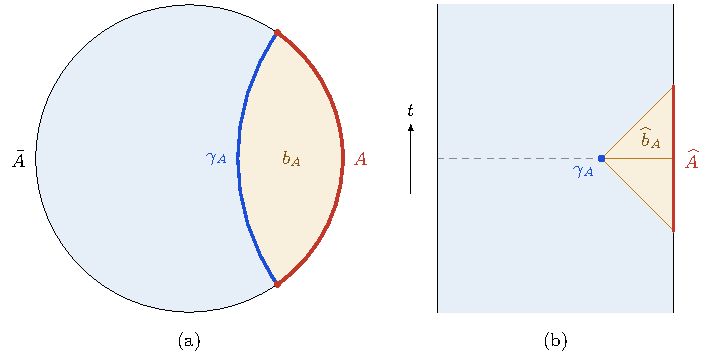
\includegraphics[width=0.82\textwidth]{figs/fig_rt.pdf}
\caption{(a) A constant-time slice of AdS drawn as a disk, whose edge is the boundary: the Ryu--Takayanagi surface $\gamma_A$ (blue) is the minimal curve anchored at the endpoints of the boundary region $A$ (red), $b_A$ (gold) is the bulk region between them, and $\bar A$ is the rest of the boundary. The entropy of $A$ is $S(A)=\mathrm{Area}(\gamma_A)/4G_N+S_{\rm bulk}(b_A)=S_{\rm gen}(b_A)$. (b) A side view, with time running upward, cut through the middle of $A$: the entanglement wedge $\widehat b_A$ (gold), bounded by light rays, is the domain of dependence of $b_A$; it meets the boundary along $\widehat A$ (red), and its tip on the $t=0$ slice (dashed) is $\gamma_A$ (blue dot).}
\label{fig:rt_entanglement_wedge}
\end{figure}

The boundary construction of $X_A$ needs some care. It is used many times below, so here it is in detail.
At finite $N$ there is an ordinary von Neumann algebra $B_A^{(N)}$ of operators localized in $A$. It
satisfies $B_A^{(N)}=B_{\widehat A}^{(N)}$, where $\widehat A$ is the boundary domain of dependence of $A$.
This is the ordinary time-slice axiom. As $N\to\infty$, many operators in $B_A^{(N)}$ have no sensible limit
and drop out. The right object is built from the operators that do survive the limit in the state $\Psi$:
\[
X_A \equiv \pi_\Psi\Big(\lim_{N\to\infty,\Psi}B_A^{(N)}\Big)'' = X_{\widehat A} .
\]
Here $\pi_\Psi$ is the GNS representation. The double commutant plays the same role as in the GNS discussion
of Chapter 2: it makes the result a genuine von Neumann algebra. The equality with $X_{\widehat A}$ holds
because the finite-$N$ time-slice axiom survives the limit. The content of entanglement wedge reconstruction
is that this boundary-defined algebra equals the bulk algebra in \eqref{eq:XA_def}.

A second algebra is easier to construct. The algebra $Y_{\widehat A}$ is generated by single-trace operators
restricted to $\widehat A$. It is the single-trace algebra $Y_O$ of Chapter 6, taken for the region
$\widehat A$. Single-trace operators in any region survive the large-$N$ limit by construction, so
\begin{equation}
Y_{\widehat A} \subseteq X_A .
\label{eq:YA_in_XA}
\end{equation}
The rest of this section studies this inclusion: what $Y_{\widehat A}$ describes in the bulk, and what else
$X_A$ contains.

\subsection*{Causal wedge reconstruction: the ``easy'' part of $X_A$}

Causal wedge reconstruction is also known as HKLL reconstruction (after Hamilton, Kabat, Lifschytz, and
Lowe). It concerns the \textbf{causal wedge}
\[
C_{\widehat A}\equiv \widetilde J^+(\widehat A)\cap\widetilde J^-(\widehat A) ,
\]
where $\widetilde J^\pm$ denote the bulk causal future and past. So $C_{\widehat A}$ is the set of bulk points
that can both receive signals from $\widehat A$ and send signals to $\widehat A$. Causal wedge reconstruction
states that bulk fields in $C_{\widehat A}$ can be written directly as single-trace operators smeared over
$\widehat A$:
\begin{equation}
\Phi(X) = \int d^dx\,K_A^{(C)}(X;x)\,\pi_\Psi(O(x)), \qquad X\in C_{\widehat A},\ x\in\widehat A .
\label{eq:HKLL_region}
\end{equation}
Here $K_A^{(C)}$ is an explicit kernel. In general it is a distribution rather than a smooth function. This
is the HKLL construction of Chapter 6, now applied to a general region instead of the whole boundary.
Algebraically, it says
\[
\widetilde\M_{C_{\widehat A}} = Y_{\widehat A} .
\]
For $A$ equal to a full boundary, this is the black-hole exterior identification of Chapter 6.

The causal wedge always lies inside the entanglement wedge, $C_{\widehat A}\subseteq\widehat b_A$. This is a
standard geometric fact. It says that causal reconstruction is always more conservative than
entanglement-based reconstruction. Combine this fact with the definition \eqref{eq:XA_def} and with
$\widetilde\M_{C_{\widehat A}}=Y_{\widehat A}$. The inclusion \eqref{eq:YA_in_XA} then follows at once: it is
the algebraic image of the geometric inclusion $C_{\widehat A}\subseteq\widehat b_A$.

\subsection*{Where the rest of $X_A$ comes from: modular flow, made explicit}

The double-commutant definition fixes $X_A$ abstractly. It does not say which operators $X_A$ contains
beyond $Y_{\widehat A}$. On the gravity side, the entanglement wedge is generically strictly larger than the
causal wedge. Equality holds only in special, highly symmetric cases. So generically
$Y_{\widehat A}\subsetneq X_A$.

Here the ergodic lemma of Chapter 4 does real work. The lemma concerns two von Neumann algebras
$\N\subset\mathcal X$ and a vector that is cyclic and separating for both. It says that the modular flow of
the larger algebra $\mathcal X$, applied to the smaller algebra $\N$, generates all of $\mathcal X$.

We apply it with $\mathcal X=X_A$. Since $b_A$ is a genuine bulk local region, $\ket1_\Psi$ is cyclic and
separating for $X_A=\widetilde\M_{b_A}$. Call the corresponding modular operator $\Delta_{X_A}$. By
\eqref{eq:subregion_subalgebra}, it equals the bulk modular operator $\widetilde\Delta_{b_A}$. For the smaller
algebra we take $Y_A^\epsilon$. This is the algebra of single-trace operators smeared within a thin time band
of width $\epsilon$ around $A$. Picture a thin strip of boundary spacetime hugging the region $A$. Its causal
wedge is a thin open bulk region next to $A$, so by the Reeh--Schlieder property $\ket1_\Psi$ is still cyclic
and separating for $Y_A^\epsilon$. The lemma then says that modular flow of the \emph{full} algebra $X_A$
regenerates all of $X_A$ from this thin sliver:
\[
X_A = \Big\{\, \Delta_{X_A}^{-is}\,O_\epsilon(\vec x)\,\Delta_{X_A}^{is} \ :\ \vec x\in A,\ s\in\mathbb R
\,\Big\}'' .
\]
Here $O_\epsilon(\vec x)$ is a single-trace operator smeared over the thin band near the point $\vec x$.
\textbf{The extra operators in $X_A$, beyond single-trace operators smeared over $\widehat A$, are
single-trace operators carried along by modular flow.}

Write $O(s;\vec x)\equiv\Delta_{X_A}^{-is}\,O_\epsilon(\vec x)\,\Delta_{X_A}^{is}$ for these modular-flowed
operators. At the free-field level of the large-$N$ limit the state is Gaussian. The modular flow of a
Gaussian state maps each smeared field to another field that is again linear in the original fields. A bulk
field is itself linear in the fields. So a bulk field anywhere in the entanglement wedge, not only in the
causal wedge, can be written as
\[
\Phi(X) = \int_{-\infty}^\infty ds\int d\vec x\,K_A^{(E)}(X;s,\vec x)\,O(s;\vec x), \qquad X\in\widehat b_A .
\]
This is the entanglement-wedge generalization of the HKLL formula \eqref{eq:HKLL_region}. Formulas of this
type were first proposed on other grounds. Here their existence follows directly from modular theory. The
kernel $K_A^{(E)}$ is in general not known in closed form.

A related result, the \textbf{JLMS relation} (Jafferis, Lewkowycz, Maldacena, and Suh, 2015), connects
boundary and bulk modular flow at large but finite $N$. In the strict large-$N$ limit it reduces to the
statement $\Delta_{X_A}=\widetilde\Delta_{b_A}$ used above. The JLMS relation is often quoted without
derivation. The box below shows how it fits together with two other holographic results.

\begin{keyresult}[: The JLMS relation and modular flow]
\textbf{Statement (JLMS).} Let $A$ be a boundary spatial region, with entanglement wedge $b_A$ bounded by the
RT surface $\gamma_A$. Work on the code subspace, the space of semiclassical states around a fixed
background. Let $\sigma$ be a reference state in it, and write the modular Hamiltonians with density matrices
(at large but finite $N$, with a short-distance cutoff where needed):
\[
H_A \equiv -\log\sigma_A , \qquad H_{\text{bulk}} \equiv -\log\sigma_{b_A} .
\]
\begin{enumerate}
\item The boundary and bulk modular Hamiltonians obey an operator identity on the code subspace,
\[
H_A = \frac{\hat A[\gamma_A]}{4G_N} + H_{\text{bulk}} + \mathcal{O}(G_N) ,
\]
where $\hat A[\gamma_A]$ is the area operator of the RT surface. (The area term is understood to include the
local terms on $\gamma_A$, such as counterterms, that also appear in the FLM formula below.)
\item For any bulk operator $\Phi \in \widetilde\M_{b_A}$ in the entanglement wedge,
\[
\Delta_A^{-is}\,\Phi\,\Delta_A^{is} = \widetilde\Delta_{b_A}^{-is}\,\Phi\,\widetilde\Delta_{b_A}^{is} .
\]
In words, boundary modular flow acts on every entanglement-wedge operator exactly as bulk modular flow does.
\end{enumerate}

\textbf{How the pieces fit.} The argument below takes two inputs: the equality of bulk and boundary relative
entropies (step 1), and the FLM formula (step 3). JLMS originally argued in the other direction. They started
from FLM, derived the modular Hamiltonian identity, and then obtained the equality of relative entropies.
Given FLM, the two statements are equivalent at this order. So the argument shows how the pieces fit
together. It is not a derivation from first principles.
\begin{enumerate}[leftmargin=*]
\item \textbf{Relative entropy equality.}
Let $\sigma$ be a reference background state, such as the global vacuum or the thermofield double. Let $\rho$
be any nearby excited state in the code subspace. The input is that the relative entropy of the boundary
region $A$ equals that of the bulk entanglement wedge $b_A$, up to small corrections:
\[
D(\rho_A \| \sigma_A) = D(\rho_{\text{bulk}} \| \sigma_{\text{bulk}}) + \mathcal{O}(G_N) .
\]

\item \textbf{Relative entropy in terms of modular Hamiltonians.}
For any two density matrices, with $H^\sigma\equiv-\log\sigma$,
\begin{align}
D(\rho\|\sigma) &\eqstep{1} \Tr(\rho\log\rho) - \Tr(\rho\log\sigma) \notag\\
&\eqstep{2} -S(\rho) + \Braket{H^\sigma}_\rho . \notag
\end{align}
\stepwhy{1}{the definition of relative entropy.}\quad
\stepwhy{2}{$S(\rho)=-\Tr(\rho\log\rho)$, and $-\log\sigma=H^\sigma$.}

Applied to the boundary state and to the bulk state in the entanglement wedge, this gives
\begin{align*}
D(\rho_A \| \sigma_A) &= -S(\rho_A) + \Braket{H_A}_\rho , \\
D(\rho_{\text{bulk}} \| \sigma_{\text{bulk}}) &= -S(\rho_{\text{bulk}}) + \Braket{H_{\text{bulk}}}_\rho .
\end{align*}

\item \textbf{The FLM formula.}
The Faulkner--Lewkowycz--Maldacena (FLM) formula is the quantum-corrected RT formula. It says that the
boundary entanglement entropy equals the bulk generalized entropy, at leading and first subleading order:
\[
S(\rho_A) = \Braket{\frac{\hat A[\gamma_A]}{4G_N}}_\rho + S(\rho_{\text{bulk}}) + \mathcal{O}(G_N) .
\]

\item \textbf{Cancellation of the bulk entropy.}
Start from the boundary relative entropy and use steps 2, 3, and 1 in turn:
\begin{align}
D(\rho_A \| \sigma_A)
&\eqstep{1} -S(\rho_A) + \Braket{H_A}_\rho \notag\\
&\eqstep{2} -\Braket{\frac{\hat A[\gamma_A]}{4G_N}}_\rho - S(\rho_{\text{bulk}}) + \Braket{H_A}_\rho
  + \mathcal O(G_N) \notag\\
&\eqstep{3} -S(\rho_{\text{bulk}}) + \Braket{H_{\text{bulk}}}_\rho + \mathcal O(G_N) . \notag
\end{align}
\stepwhy{1}{step 2 applied to the boundary state.}\quad
\stepwhy{2}{insert the FLM formula of step 3 for $S(\rho_A)$.}\quad
\stepwhy{3}{the relative entropy equality of step 1, with the bulk relative entropy written out using
step 2.}

The bulk entropy $S(\rho_{\text{bulk}})$ appears on both sides of the last equality, so it cancels.
Rearranging what is left gives
\[
\Braket{H_A}_\rho = \Braket{\frac{\hat A[\gamma_A]}{4G_N} + H_{\text{bulk}}}_\rho + \mathcal O(G_N) .
\]

\item \textbf{From expectation values to an operator identity.}
This equality holds for \emph{every} state $\rho$ in the code subspace. The expectation values of a Hermitian
operator in all density matrices supported on a subspace determine that operator's restriction to the
subspace. So the two operators agree on the code subspace:
\[
H_A = \frac{\hat A[\gamma_A]}{4G_N} + H_{\text{bulk}} + \mathcal{O}(G_N) .
\]

\item \textbf{Action on bulk operators.}
Let $\Phi \in \widetilde\M_{b_A}$ be an operator localized in the interior of the entanglement wedge. The RT
surface $\gamma_A = \partial b_A$ is the edge of the wedge, so it is spacelike separated from $\Phi$. At
leading order the area operator therefore commutes with $\Phi$:
\[
\left[\frac{\hat A[\gamma_A]}{4G_N}, \, \Phi\right] = 0 .
\]
Now compute the commutator of $\Phi$ with the boundary modular Hamiltonian:
\begin{align}
[H_A, \, \Phi] &\eqstep{1} \left[\frac{\hat A[\gamma_A]}{4G_N} + H_{\text{bulk}}, \, \Phi\right]
\eqstep{2} [H_{\text{bulk}}, \, \Phi] . \notag
\end{align}
\stepwhy{1}{the operator identity of step 5, at leading order.}\quad
\stepwhy{2}{the commutator is linear, and the area term commutes with $\Phi$.}

The operator $[H_{\text{bulk}},\Phi]$ again lies in $\widetilde\M_{b_A}$, so the same step applies to it.
Hence all nested commutators agree, $[H_A,[H_A,\dots[H_A,\Phi]]]=[H_{\text{bulk}},[H_{\text{bulk}},\dots
[H_{\text{bulk}},\Phi]]]$. Summing the exponential series of nested commutators then gives, formally,
\[
e^{is H_A}\, \Phi\, e^{-is H_A} = e^{is H_{\text{bulk}}}\, \Phi\, e^{-is H_{\text{bulk}}} .
\]
Finally, the full modular operator is $\Delta_A=\sigma_A\otimes\sigma_{\bar A}^{-1}$. Its $\sigma_{\bar A}$
factor commutes with $\Phi$, so $\Delta_A^{-is}\Phi\Delta_A^{is}=\sigma_A^{-is}\Phi\sigma_A^{is}
=e^{isH_A}\Phi e^{-isH_A}$. The same holds in the bulk. Therefore
\[
\Delta_A^{-is}\,\Phi\,\Delta_A^{is} = \widetilde\Delta_{b_A}^{-is}\,\Phi\,\widetilde\Delta_{b_A}^{is} .
\qquad \blacksquare
\]
\end{enumerate}
\end{keyresult}

When is the causal-wedge piece already everything, so that $X_A=Y_{\widehat A}$? This happens exactly when the
bulk modular flow of $b_A$ acts \emph{geometrically}. That means it acts as a pointwise coordinate
transformation, like the Rindler-wedge boost of Chapter 4. A flow of this kind maps operators localized in
$\widehat A$ to operators that are still localized in $\widehat A$, so it generates nothing new. This happens
for a half-space or a spherical region in the vacuum, and for the full boundary in the thermofield double.
These are exactly the cases already worked out explicitly. In them $X_A=Y_{\widehat A}$ and
$\widehat b_A=C_{\widehat A}$ hold exactly. In general, though, modular flow is \emph{not} geometric, and the
inclusion \eqref{eq:YA_in_XA} is strict.

\begin{physconnect}[: Modular Flow and Operator Generation]
\textbf{You have already met a finite-dimensional version of this object in Chapter 4.} There, the modular
flow of a single entangled pair, $\sigma_s(A)=\rho_R^{-is}A\rho_R^{is}$, was an ordinary unitary conjugation.
You worked it out explicitly on a $4\times4$ matrix. Here the same object, the modular flow of a boundary
algebra, does something with no finite-dimensional analogue. Starting from a small algebra, it generates
operators that were not in that algebra, and in fact the whole larger algebra. This is possible only because
the algebras involved are infinite-dimensional (here, type $\mathrm{III}_1$).

In finite dimensions the ergodic lemma has no content. Suppose $\N\subset\M$ act on a finite-dimensional
Hilbert space $\HH$, and a vector $\ket\Omega$ is cyclic for $\N$ and separating for $\M$. Because
$\ket\Omega$ is separating for $\M$, the map $x\mapsto x\ket\Omega$ is injective on $\M$, so
$\dim\M\le\dim\HH$. Because $\ket\Omega$ is cyclic for $\N$, the vectors $x\ket\Omega$ with $x\in\N$ fill all
of $\HH$, so $\dim\N\ge\dim\HH$. Together these give $\dim\N\ge\dim\M$, and so $\N=\M$. In finite dimensions
a proper subalgebra can never share such a vector with the larger algebra. There is nothing left for
modular flow to fill in.

In infinite dimensions the situation is different. By the Reeh--Schlieder property, a small subalgebra, such
as the thin sliver above, can have the same cyclic and separating vector as the larger algebra. Modular flow
can then sweep out the entire larger algebra from the sliver. This is the ``ergodic'' lemma of Chapter 4, now
doing physical work: it builds an entire entanglement wedge, or a black-hole interior, out of a thin sliver of
boundary time. The definition of modular flow has not changed. What changed is that infinite dimensions let it
do something a finite matrix conjugation cannot.
\end{physconnect}

\subsection*{Two logically distinct sources of type $\mathrm{III}_1$}

Both $X_A$ and $Y_{\widehat A}$ are type $\mathrm{III}_1$. This property can have two different physical
origins, and it helps to keep them apart.

The first origin is the one met in Chapter 4. For a continuum quantum field theory at finite $N$, the local
algebra $B_A^{(N)}$ is already type $\mathrm{III}_1$. The cause is the infinite amount of \emph{short}-range
entanglement across the boundary $\partial A$. In the bulk, this matches the fact that the RT surface reaches
the AdS boundary, which is at infinite proper distance.

To isolate the second origin, put the boundary theory on a lattice. Then at any finite $N$ the algebra
$B_A^{(N)}$ is type I: it is an algebra of finite matrices, with minimal projections. Yet $X_A$ and
$Y_{\widehat A}$, defined through the large-$N$ limit, are \emph{still} type $\mathrm{III}_1$. So their type
$\mathrm{III}_1$ property does not come from the type of $B_A^{(N)}$ before the limit. It comes from an
infinite amount of \emph{long}-range entanglement between $A$ and its complement, which appears only in the
strict $N\to\infty$ limit. In the bulk, this matches the infinite short-range entanglement of bulk fields
across the RT surface $\gamma_A$ (or, for $Y_{\widehat A}$, across the edge $\chi_{\widehat A}$ of the causal
wedge).

So two independent mechanisms produce the same type of algebra, at two different stages of the same
construction: finite $N$, and the strict $N\to\infty$ limit.

The same picture gives an algebraic way to locate the RT surface. Near $\gamma_A$, bulk modular flow acts as a
local boost. This is the local-Rindler argument of Chapter 4, applied at the RT surface. The surface
$\gamma_A$ is the fixed (``invariant'') set of that boost. By the JLMS relation, boundary modular flow acts on
wedge operators as bulk modular flow does. So \textbf{the RT surface can be characterized, without assuming a
bulk metric, as the asymptotic fixed-point set of the boundary modular flow}. This gives an algebraic
restatement of the procedure for finding the RT surface.

\subsection*{Extended gravitational systems: algebra without any geometry to point to}

The entanglement-wedge and causal-wedge story extends beyond geometric boundary regions. Replace $A$ by
\emph{any} von Neumann subalgebra $\M$ of the boundary theory. Then define $X_\M$ by the direct analogue of the
double-commutant definition of $X_A$. This definition makes sense even when there is no bulk geometric
picture at all.

One can go further. Couple a gravitational sector $B$ (which has its own boundary dual) to an ordinary
non-gravitational sector $R$. For example, $R$ could be radiation that has already escaped to infinity. For
any subsystem $Q$ of the combined system $B\cup R$, define two algebras:
\begin{itemize}
\item the entanglement wedge algebra $X_Q\equiv\lim_{G_N\to0,\Psi}B_Q$, whether or not it has a geometric
meaning;
\item the causal wedge algebra $Y_Q$, the algebra of $Q$'s ordinary low-energy effective description.
\end{itemize}
This abstraction is exactly what the evaporating-black-hole discussion later in this chapter needs. There,
$Q$ will be the emitted Hawking radiation.

\section{Quantum informational aspects of entanglement wedge reconstruction}

\subsection*{Superadditivity, and its boundary origin}

\textbf{Entanglement wedge nesting} is a standard geometric fact, which follows from the extremality of RT
surfaces. For boundary regions $A_1\subseteq A_2$, the entanglement wedges satisfy
$\widehat b_{A_1}\subseteq\widehat b_{A_2}$. Algebraically this is just $X_{A_1}\subseteq X_{A_2}$, which
follows immediately from $A_1\subseteq A_2$ and the definition of $X_A$.

Nesting has a direct geometric consequence. For two regions $A_1,A_2$ on one Cauchy slice,
\[
b_{A_1}\cup b_{A_2} \subseteq b_{A_1\cup A_2}, \qquad b_{A_1\cap A_2}\subseteq b_{A_1}\cap b_{A_2} .
\]
This is a consequence of nesting, not an extra assumption. In words, the entanglement wedge of a union is at
least as big as the union of the entanglement wedges, and generically it is strictly bigger. This is
\textbf{superadditivity of entanglement wedges}. Two AdS$_3$ examples make it concrete: two overlapping
boundary intervals, and two disjoint intervals placed close together. In both cases the RT surface of the
union ``jumps'' and encloses visibly more bulk than the two pieces do separately. Translated through the
definition \eqref{eq:XA_def}, superadditivity becomes a statement purely about boundary algebras:
\begin{equation}
X_{A_1}\vee X_{A_2} \subseteq X_{A_1\cup A_2}, \qquad X_{A_1\cap A_2}\subseteq X_{A_1}\wedge X_{A_2} .
\label{eq:superadditivity_alg}
\end{equation}

Compare this with the additivity axiom of Chapter 4 for an ordinary relativistic quantum field theory at
finite $N$. For topologically trivial regions, that axiom says $B_{A_1}^{(N)}\vee B_{A_2}^{(N)}
=B_{A_1\cup A_2}^{(N)}$. \textbf{For the inclusions \eqref{eq:superadditivity_alg} to be strict, ordinary
additivity has to fail in the strict large-$N$ limit.} One can show that it does fail in the two AdS$_3$
examples above. The argument uses a classic result of Araki. It identifies $X_{A_1}\vee X_{A_2}$ concretely as
the algebra of single-trace operators in a specific larger causal region. That algebra is strictly smaller
than $X_{A_1\cup A_2}$. (We quote this computation without reproducing it.) \textbf{Superadditivity of
entanglement wedges is the bulk geometric image of the failure of additivity for boundary algebras in the
strict large-$N$ limit.} Algebras of local regions are then no longer ``locally generated'' in the way the
algebras of an ordinary finite-$N$ quantum field theory are.

Haag duality, by contrast, survives. Assume it holds for the bulk algebras, $\widetilde\M_{b'}=
\widetilde\M_b'$. For a pure global state, $A$ and its complement $\bar A$ share the same RT surface. So
$b_{\bar A}$ is the bulk complement $b_A'$. Then Haag duality holds in the large-$N$ limit:
\[
X_{A}' = X_{\bar A} .
\]
The single-trace algebra $Y_{\widehat A}$ behaves in the opposite way. It is additive by construction, but in
general it does \emph{not} satisfy Haag duality.

\subsection*{Quantum error correction, made precise}

Entanglement wedge reconstruction has long been interpreted in the language of quantum error correction.
All the information in $b_A$ can be recovered from boundary data on $A$ alone. So this information is
protected against ``erasing'' the complementary region $\bar A$ entirely. Superadditivity makes this more
precise and checkable.

Take an operator $\Phi(X)$ at a point $X$ in a bulk region $b$. Suppose $b$ lies in the \emph{intersection}
of the entanglement wedges of two different boundary regions $A$ and $\widetilde A$, but outside the
entanglement wedge of $A\cap\widetilde A$. Picture two overlapping boundary intervals. Their wedges overlap
in a bulk region that reaches deeper than the wedge of their small common piece. Now use the HKLL-type formula
\eqref{eq:HKLL_region}. For concreteness, take a case in the vacuum sector (GNS representation $\pi_\Omega$)
where the causal and entanglement wedges coincide for both $A$ and $\widetilde A$. Then
\begin{equation}
\Phi(X) = \pi_\Omega(O_A(X)) = \pi_\Omega(O_{\widetilde A}(X)) .
\label{eq:double_reconstruction}
\end{equation}
Here $O_A(X)$ and $O_{\widetilde A}(X)$ are two \emph{different} boundary operators. They are built from
different single-trace data, smeared over $A$ and over $\widetilde A$ respectively. Yet they coincide once
represented on the GNS Hilbert space. In fact there is an infinite family of such reconstructions, one for
every boundary region whose entanglement wedge contains $b$.

\textbf{So a bulk degree of freedom $\Phi(X)$ in $b$ cannot be assigned to any one boundary region. It is
encoded collectively and redundantly across the boundary system. This is the defining feature of a quantum
error-correcting code.} This redundancy follows from superadditivity \eqref{eq:superadditivity_alg}. It is not
an extra postulate added to the holographic dictionary.

\subsection*{Worked calculation: a three-qubit toy code}

To see this redundancy in elementary matrix algebra, we work through a small toy code with three qubits. It is
a simplified cousin of the three-qutrit code of Almheiri, Dong, and Harlow, which is the standard example. The
qubit version is not perfect, as we will see, but it already shows the key mechanism.

Let the bulk logical state be a single qubit at the center of the disk:
\[
\ket{\psi}_L = \alpha \ket{0}_L + \beta \ket{1}_L, \qquad |\alpha|^2 + |\beta|^2 = 1 .
\]
The boundary consists of three physical qubits $A, B, C$. The encoding isometry
$V: \mathbb{C}^2 \to (\mathbb{C}^2)^{\otimes 3}$ is defined by
\[
\ket{0}_L \mapsto \frac{1}{\sqrt{2}}\big(\ket{000} + \ket{111}\big), \qquad
\ket{1}_L \mapsto \frac{1}{\sqrt{2}}\big(\ket{100} + \ket{011}\big) .
\]
The four basis states that appear are distinct, so the two code states are orthonormal and $V$ is an
isometry. The encoded boundary state is
\begin{align*}
\ket{\Psi(\alpha,\beta)}
&= \frac{\alpha}{\sqrt{2}}\big(\ket{000}_{ABC} + \ket{111}_{ABC}\big) \\
&\quad + \frac{\beta}{\sqrt{2}}\big(\ket{100}_{ABC} + \ket{011}_{ABC}\big) .
\end{align*}

\textbf{A single qubit.} Compute the reduced density matrix of qubit $C$ by tracing out qubits $A$ and $B$:
\[
\rho_C = \Tr_{AB}\big(\ket{\Psi}\bra{\Psi}\big) = \sum_{a,b \in \{0,1\}} \braket{ab|\Psi}\braket{\Psi|ab} .
\]
Here $\braket{ab|\Psi}$ is a (unnormalized) state of qubit $C$. The four overlaps with the basis states of
$AB$ are
\begin{align*}
\braket{00|\Psi} &= \tfrac{\alpha}{\sqrt{2}}\ket{0}_C , &
\braket{00|\Psi}\braket{\Psi|00} &= \tfrac{|\alpha|^2}{2}\ket{0}\bra{0}_C , \\
\braket{10|\Psi} &= \tfrac{\beta}{\sqrt{2}}\ket{0}_C , &
\braket{10|\Psi}\braket{\Psi|10} &= \tfrac{|\beta|^2}{2}\ket{0}\bra{0}_C , \\
\braket{11|\Psi} &= \tfrac{\alpha}{\sqrt{2}}\ket{1}_C , &
\braket{11|\Psi}\braket{\Psi|11} &= \tfrac{|\alpha|^2}{2}\ket{1}\bra{1}_C , \\
\braket{01|\Psi} &= \tfrac{\beta}{\sqrt{2}}\ket{1}_C , &
\braket{01|\Psi}\braket{\Psi|01} &= \tfrac{|\beta|^2}{2}\ket{1}\bra{1}_C .
\end{align*}
Each $AB$ basis state picks out exactly one of the four terms of $\ket\Psi$. Summing:
\begin{align}
\rho_C &\eqstep{1} \left(\frac{|\alpha|^2 + |\beta|^2}{2}\right)\ket{0}\bra{0}_C
+ \left(\frac{|\alpha|^2 + |\beta|^2}{2}\right)\ket{1}\bra{1}_C \notag\\
&\eqstep{2} \frac{1}{2}\begin{pmatrix} 1 & 0 \\ 0 & 1 \end{pmatrix} = \frac{1}{2}\id_2 . \notag
\end{align}
\stepwhy{1}{add the four terms of the table, grouping the two that multiply $\ket0\bra0_C$ and the two that
multiply $\ket1\bra1_C$.}\quad
\stepwhy{2}{normalization of the logical state, $|\alpha|^2+|\beta|^2=1$.}

So $\rho_C$ is proportional to the identity matrix. It does not depend on the logical amplitudes $\alpha$ and
$\beta$ at all. The same four-overlap computation for qubit $B$ (now tracing out $A$ and $C$) gives the same
answer, $\rho_B=\tfrac12\id_2$. So qubit $B$ alone and qubit $C$ alone each contain \textbf{no} information
about the central bulk qubit. Qubit $A$ is different. The same computation gives
$\rho_A=\tfrac12\id_2+\Re(\alpha\beta^*)\,X_A$, which does depend on the logical state. (These three reduced
density matrices were also checked numerically.) Three qubits are too few for a code in which \emph{every}
single qubit is blind to the logical information. The perfect version of this toy code uses three qutrits
(three-level systems) instead.

\textbf{Two qubits.} Now consider reconstructing logical operators on \emph{two} qubits, a boundary subregion
of size 2.
\begin{enumerate}
\item \textbf{Logical $Z_L = \ket{0}_L\bra{0} - \ket{1}_L\bra{1}$}.
Define the boundary operator $Z_{AB} \equiv Z_A \otimes Z_B$ acting on region $AB$. Then
\begin{align}
(Z_A \otimes Z_B \otimes \id_C)\ket{0}_L &\eqstep{1} \tfrac{1}{\sqrt{2}}\big( (+1)(+1)\ket{000}
+ (-1)(-1)\ket{111}\big) \notag\\
&\eqstep{2} \ket{0}_L , \notag\\
(Z_A \otimes Z_B \otimes \id_C)\ket{1}_L &\eqstep{1} \tfrac{1}{\sqrt{2}}\big( (-1)(+1)\ket{100}
+ (+1)(-1)\ket{011}\big) \notag\\
&\eqstep{2} -\ket{1}_L . \notag
\end{align}
\stepwhy{1}{$Z$ gives $+1$ on $\ket0$ and $-1$ on $\ket1$, applied to qubits $A$ and $B$; the identity leaves
qubit $C$ alone.}\quad
\stepwhy{2}{multiply the signs and compare with the encoding of $\ket0_L$ and $\ket1_L$.}

Hence $(Z_{AB} \otimes \id_C)\ket{\psi}_L = Z_L\ket{\psi}_L$.
\item \textbf{Logical $X_L = \ket{0}_L\bra{1} + \ket{1}_L\bra{0}$}.
Define the boundary operator $X_{AB} \equiv X_A \otimes \id_B$ on region $AB$. (It acts nontrivially only on
qubit $A$.) Then
\begin{align}
(X_A \otimes \id_B \otimes \id_C)\ket{0}_L &\eqstep{1} \tfrac{1}{\sqrt{2}}\big(\ket{100} + \ket{011}\big)
\eqstep{2} \ket{1}_L , \notag\\
(X_A \otimes \id_B \otimes \id_C)\ket{1}_L &\eqstep{1} \tfrac{1}{\sqrt{2}}\big(\ket{000} + \ket{111}\big)
\eqstep{2} \ket{0}_L . \notag
\end{align}
\stepwhy{1}{$X$ flips qubit $A$, $\ket0\leftrightarrow\ket1$, and leaves $B$ and $C$ alone.}\quad
\stepwhy{2}{compare with the encoding of $\ket1_L$ and $\ket0_L$.}

Hence $(X_{AB} \otimes \id_C)\ket{\psi}_L = X_L\ket{\psi}_L$.
\end{enumerate}

The logical $X_L$ can also be reconstructed on the complementary region $BC$, as
$X_{BC} \equiv \id_A \otimes X_B \otimes X_C$:
\begin{align}
(\id_A \otimes X_B \otimes X_C)\ket{0}_L &\eqstep{1} \tfrac{1}{\sqrt{2}}\big(\ket{011} + \ket{100}\big)
\eqstep{2} \ket{1}_L , \notag\\
(\id_A \otimes X_B \otimes X_C)\ket{1}_L &\eqstep{1} \tfrac{1}{\sqrt{2}}\big(\ket{111} + \ket{000}\big)
\eqstep{2} \ket{0}_L . \notag
\end{align}
\stepwhy{1}{flip qubits $B$ and $C$ in each basis state: $\ket{000}\to\ket{011}$, $\ket{111}\to\ket{100}$,
$\ket{100}\to\ket{111}$, $\ket{011}\to\ket{000}$.}\quad
\stepwhy{2}{compare with the encoding.}

Flipping only qubit $B$ would not work: $X_B\ket0_L=\tfrac1{\sqrt2}(\ket{010}+\ket{101})$ lies outside the
code subspace. Both $X_A \otimes \id_B \otimes \id_C$ and $\id_A \otimes X_B \otimes X_C$ act on the code
subspace as the central bulk operator $\Phi(0) = X_L$. Yet they are supported on disjoint, complementary
boundary regions ($A$ versus $BC$). The same kind of redundancy holds for $Z_L$. Repeating the sign computation
above with $Z$ on qubits $A$ and $C$ shows that $Z_A\otimes\id_B\otimes Z_C$ also acts as $Z_L$. So $Z_L$ can
be built on $AB$ or on $AC$.

To summarize: each of the regions $AB$ and $AC$ reconstructs the full logical algebra (both $X_L$ and $Z_L$).
The region $BC$ does not. It reconstructs $X_L$ but not $Z_L$. The reason is that every operator on $BC$
commutes with $X_A$, which acts as $X_L$, so the logical action of any operator on $BC$ must commute with
$X_L$. (A search over all three-qubit Pauli strings confirms this list of reconstructions numerically.) In the
three-qutrit code, by contrast, any two of the three qutrits reconstruct every logical operator. Even in this
imperfect qubit version, the same logical operator lives on several different boundary regions. This is the
algebraic mechanism of holographic error correction.

One caveat about this picture. The ``bulk Hilbert space as a code subspace'' picture from quantum error
correction is literally meaningful only at finite $N$. The bulk semiclassical Hilbert space, on the other hand,
is only precisely defined at $N=\infty$. So holographic error correction is better understood as a framework
connecting the two regimes. Any finite-$N$ code is necessarily only \emph{approximately} isometric, and should
not be read as a literal, exact implementation of the holographic dictionary.

\begin{physconnect}[: Redundant Purifications and Code Subspaces]
The operator $\Phi(X)$ can be written using completely different boundary data (region $A$ or region
$\widetilde A$), while remaining, in every observable sense, the same operator. This is a large-scale version
of a fact you already know from ordinary quantum information: \textbf{purification is never unique.}

Take a single mixed qubit, $\rho=\mathrm{diag}(0.7,0.3)$. One purification uses a second qubit as the
ancilla, $\ket\Psi_1=\sqrt{0.7}\ket{00}+\sqrt{0.3}\ket{11}$. A completely different one uses, say, a 3-level
ancilla, $\ket\Psi_2=\sqrt{0.7}\ket{0}\ket{a}+\sqrt{0.3}\ket{1}\ket{b}$, for any orthonormal $\ket a,\ket b$ in
the bigger ancilla space. Trace out the ancilla in either case and you get back the same $\rho$. You can check
this directly from the definition of the partial trace: the result depends only on the Schmidt coefficients
$\sqrt{0.7},\sqrt{0.3}$, not on which ancilla states carry them. \textbf{No measurement confined to the
original qubit can tell you which purification, meaning which ancilla entangled in which way, is ``really''
on the other side.} The information is present, but it is not attached to any single, canonical description of
the environment. It is attached only to the reduced state itself.

The double reconstruction \eqref{eq:double_reconstruction} works the same way, at the scale of an entire
holographic boundary instead of one ancilla qubit. The observable content of $\Phi(X)$ on the GNS Hilbert space
is fixed. But the choice of boundary data used to build it (region $A$ or region $\widetilde A$) is as
non-unique as the choice of ancilla above. As in the qubit example, no measurement of the reconstructed
operator itself can tell you which region did the reconstructing. What is new here, with no counterpart in the
single-qubit example, is the \emph{physical} content of that redundancy. It is not just a bookkeeping fact about
how $\rho$ can be written as a partial trace. Superadditivity \eqref{eq:superadditivity_alg} ties it to real
bulk geometry. It turns ``purification is not unique'' into ``a bulk region is stored redundantly enough to
survive the erasure of a boundary subregion.'' That is the operational content of a quantum error-correcting
code.
\end{physconnect}

\section{An algebraic formulation of entanglement islands}

\subsection*{The island phenomenon, restated algebraically}

The \textbf{entanglement island} phenomenon is central to modern derivations of the Page curve for an
evaporating black hole. It says the following. After the Page time $t_P$, the black-hole interior stops being
part of the black hole's own entanglement wedge. Instead it becomes part of the entanglement wedge of the
emitted radiation $R$.

Split the full system into the black-hole boundary theory $B$ and the radiation $R$
(Figure~\ref{fig:page_curve_islands}(b)). Before $t_P$, the minimal quantum extremal surface for $B$ is empty.
So $B$'s entanglement wedge is the whole Cauchy slice: the interior $I$ and the exterior $O$ together. After
$t_P$, a new, nontrivial quantum extremal surface $\alpha$ takes over, and $B$'s entanglement wedge shrinks to
the exterior $O$ alone. Algebraically,
\[
X_B = \begin{cases} \widetilde\M_O\vee\widetilde\M_I & t<t_P , \\ \widetilde\M_O & t>t_P . \end{cases}
\]
Since $B\cup R$ is the whole system, once $\widetilde\M_I$ drops out of $X_B$ it must appear in $R$'s
description instead. We use the entanglement-wedge algebra $X_R$ and the causal-wedge algebra $Y_R$ from the
discussion of extended gravitational systems earlier in this chapter. The transfer is then stated precisely as
\[
X_R = \begin{cases} Y_R & t<t_P , \\ Y_R\vee\widetilde\M_I & t>t_P . \end{cases}
\]

\begin{figure}[htbp]
\centering
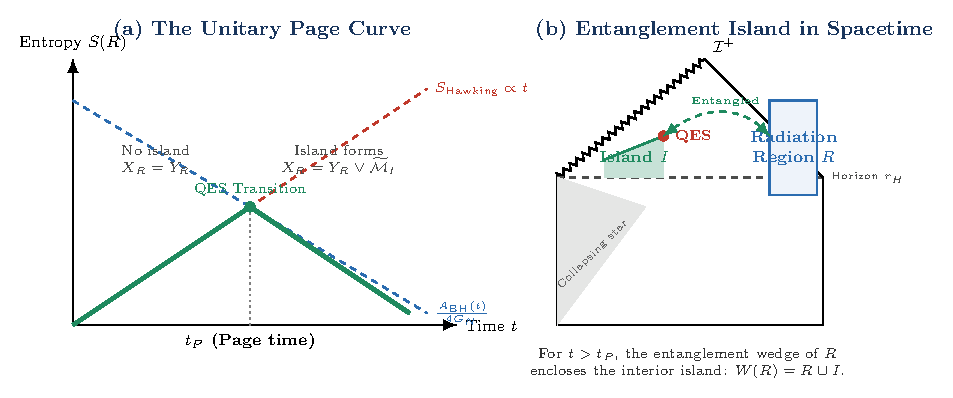
\includegraphics[width=0.95\textwidth]{figs/fig_page_curve_islands.pdf}
\caption{(a) Entropy of the radiation $R$ against time. Hawking's no-island answer (dashed red after $t_P$) keeps growing and the black hole's area term $A_{\text{BH}}/4G_N$ (dashed blue before $t_P$) keeps shrinking; the true entropy (green) follows the smaller of the two, turning over at the Page time $t_P$. (b) Penrose diagram of a black hole that forms from a collapsing star (gold) and evaporates completely, drawn after~\cite{AHMST}. The dashed red line is the event horizon and the zigzag the singularity; after the evaporation ends, the centre $r=0$ continues straight up. The dotted curve separates the region near the black hole, described by $B$, from the far region where the radiation collects (for an AdS black hole this is the boundary to which the bath is attached). On a Cauchy slice after $t_P$, the quantum extremal surface (red dot) lies just inside the horizon. The island $I$ (green) behind it joins the radiation region $R$ (blue) in the radiation's entanglement wedge, while the exterior $O$ between the red dot and the dotted curve belongs to $B$.}
\label{fig:page_curve_islands}
\end{figure}

This lets you \emph{detect} an island using only data intrinsic to the radiation system, with no reference to
$B$ at all. Define
\[
I_R \equiv Y_R'\cap X_R .
\]
These are the operators in $X_R$ that commute with every operator in $Y_R$. For $t>t_P$, this intersection is
exactly $\widetilde\M_I$. An island exists exactly when the intersection is nontrivial, that is, larger than
the multiples of the identity. In that case there are operators that survive the semiclassical limit but lie
outside $R$'s ordinary low-energy effective description. As with $X_A$ versus $Y_{\widehat A}$ above, these
extra operators are generated from $Y_R$ by the modular flow of $X_R$. It is the same mechanism once more.
The same definition, $I_Q\equiv Y_Q'\cap X_Q$, applies to any subsystem $Q$ of an extended gravitational
system, not just to radiation. An island for $Q$ is whatever survives the semiclassical limit but sits outside
$Q$'s own low-energy description.

Now return to an ordinary boundary region $A$, so that $Y_Q=Y_{\widehat A}$. Then the island algebra $I_A$
consists of the operators in $X_A$ that commute with all of $Y_{\widehat A}$. These are the operators that
modular flow adds to $Y_{\widehat A}$. Geometrically, they belong to the part of the entanglement wedge $b_A$
lying outside the causal wedge. Write $c_{\widehat A}$ for the part of $b_A$ inside the causal wedge. Then
$b_A=c_{\widehat A}\cup i_A$. This is an ordinary geometric decomposition: a causal-wedge part next to the
boundary, plus a deeper leftover piece $i_A$ between the causal wedge and the RT surface. It gives
\[
X_A=Y_{\widehat A}\vee\widetilde\M_{i_A}, \qquad I_A=\widetilde\M_{i_A} .
\]
So, in this language, an island is exactly the piece of an entanglement wedge that causal-wedge (HKLL)
reconstruction alone can never reach.

\begin{keyresult}[: Derivation of the Page Curve from the Quantum Extremal Island Rule]
\textbf{The island rule for radiation.} Consider an evaporating black hole coupled to a non-gravitational
radiation reservoir. The entropy of the radiation $R$ at boundary time $t$ is found by extremizing the
generalized entropy over candidate islands $I$, whose boundaries $\partial I$ are quantum extremal surfaces
(QES), and then taking the minimum over the extrema:
\[
S(R) = \min_{\text{QES } I} \operatorname{ext}_I \left[ \frac{\operatorname{Area}(\partial I)}{4G_N}
+ S_{\text{bulk}}(R \cup I) \right] .
\]

\textbf{The Page curve in a toy model.} The model below keeps only the features needed to see the shape of the
Page curve.
\begin{enumerate}[leftmargin=*]
\item \textbf{Evaporating black-hole geometry.}
Let the black hole form at $t = 0$ with initial horizon area $A_0$ and Bekenstein--Hawking entropy
$S_0 = A_0/4G_N$. As it radiates into the reservoir, its horizon area decreases. Let $\Gamma$ be the rate at
which its Bekenstein--Hawking entropy decreases, and take $\Gamma$ constant. (In a real evaporating black hole
the rate changes with time; a constant rate is a simplification.) Then
\[
S_{\text{BH}}(t) \equiv \frac{A_{\text{BH}}(t)}{4G_N} = S_0 - \Gamma t, \qquad t \in [0, t_{\text{evap}}] ,
\]
where $t_{\text{evap}} = S_0/\Gamma$ is the total evaporation time.

\item \textbf{Saddle 1: no island ($I = \emptyset$).}
For $I = \emptyset$ there is no boundary, $\partial I = \emptyset$, so $\operatorname{Area}(\partial I) = 0$.
The generalized entropy reduces to the bulk field-theory entropy of the radiation:
\[
S_{\text{no-island}}(R) = S_{\text{bulk}}(R) .
\]
In Hawking's semiclassical calculation, each outgoing quantum $c_k$ in the radiation is entangled with an
infalling partner mode $b_k$ behind the horizon:
\[
\ket{\text{Hawking pair}}_k \approx \frac{1}{\sqrt{2}}\big(\ket{0}_{c_k}\ket{0}_{b_k}
+ \ket{1}_{c_k}\ket{1}_{b_k}\big) .
\]
The reservoir $R$ collects only the outgoing quanta $c_k$. The partners $b_k$ stay behind the horizon. So
tracing them out leaves $R$ in a mixed state, and each new pair adds to its entropy. In the toy model we assume
that the radiation entropy grows at the same rate $\Gamma$ at which the black-hole entropy falls. (For a real
black hole the two rates differ by a factor of order one. This moves the crossing point below, but not the
shape of the curve.) Then
\[
S_{\text{no-island}}(R) = \int_0^t dt' \, \frac{dS_{\text{rad}}}{dt'} = \Gamma t .
\]
This grows without bound as $t$ increases. Eventually it exceeds the Bekenstein--Hawking entropy of the
remaining black hole. But a black hole with entropy $S_{\text{BH}}$ can be entangled with the radiation by at
most $S_{\text{BH}}$. This conflict is the \textbf{Hawking information paradox}.

\item \textbf{Saddle 2: an island ($I \ne \emptyset$).}
A second, non-empty extremum appears. Its boundary $\partial I$ is a quantum extremal surface located just
inside the event horizon. Its displacement from the horizon vanishes as $G_N\to0$. The region $I$ covers the
black-hole interior behind the horizon. The generalized entropy of this saddle is
\[
S_{\text{island}}(R) = \frac{\operatorname{Area}(\partial I)}{4G_N} + S_{\text{bulk}}(R \cup I) .
\]
Now evaluate the bulk matter entropy $S_{\text{bulk}}(R \cup I)$. The union $R \cup I$ contains \emph{both} the
outgoing Hawking quanta $c_k \in R$ \emph{and} their infalling partners $b_k \in I$. Each pair
$\ket{\text{Hawking pair}}_k$ is a pure state, so a pair lying entirely inside $R\cup I$ contributes no entropy.
The infalling and outgoing modes \textbf{purify each other}. What remains is the entropy of modes near
$\partial I$. It is of order $G_N^0$ and does not grow like $\Gamma t$:
\[
S_{\text{bulk}}(R \cup I) = \mathcal{O}(G_N^0) .
\]
So the large, steadily growing contribution is absent, and the area term dominates:
\begin{align}
S_{\text{island}}(R) &\eqstep{1} \frac{\operatorname{Area}(\partial I)}{4G_N} + \mathcal{O}(G_N^0)
\overset{(2)}{\approx} \frac{A_{\text{BH}}(t)}{4G_N} \eqstep{3} S_0 - \Gamma t . \notag
\end{align}
\stepwhy{1}{the bulk term $S_{\text{bulk}}(R\cup I)$ is only $\mathcal O(G_N^0)$, because the Hawking pairs
purify each other.}\quad
\stepwhy{2}{the quantum extremal surface sits just inside the horizon, so its area is the horizon area up to
tiny corrections, and the $\mathcal O(G_N^0)$ term is negligible next to terms of order $1/G_N$.}\quad
\stepwhy{3}{the linear decrease of the horizon area from step 1.}

\item \textbf{The Page time and the phase transition.}
By the island rule, the entropy is the smaller of the two saddle values:
\begin{align}
S(R) &\eqstep{1} \min\big\{ S_{\text{no-island}}(R), \, S_{\text{island}}(R) \big\}
\eqstep{2} \min\big\{ \Gamma t, \, S_0 - \Gamma t \big\} . \notag
\end{align}
\stepwhy{1}{the island rule: take the smallest of the extremal values.}\quad
\stepwhy{2}{substitute the two saddle values found in steps 2 and 3.}

Setting the two branches equal gives the \textbf{Page time} $t_P$:
\[
\Gamma t_P = S_0 - \Gamma t_P \implies t_P = \frac{S_0}{2\Gamma} = \frac{1}{2} t_{\text{evap}} .
\]
Over the lifetime of the black hole, the resulting entropy is
\[
S(R) = \begin{cases}
\Gamma t & t < t_P \quad (\text{no island}), \\
S_0 - \Gamma t = \frac{A_{\text{BH}}(t)}{4G_N} & t > t_P \quad (\text{island } I).
\end{cases}
\]
The early phase, with no island, is the Hawking phase. The late phase, with the interior island $I$, is the
unitary phase.
At $t = t_{\text{evap}}$, $S(R) \to 0$ as the black hole disappears. This is the value unitary evolution
requires: the final radiation is in a pure state.

\item \textbf{Algebraic translation.}
For $t < t_P$, the radiation algebra is simply $X_R = Y_R$. For $t > t_P$, the island forms, and
$X_R = Y_R \vee \widetilde\M_I$. The modular flow of $X_R$ then generates the entire interior algebra
$\widetilde\M_I$ from the radiation data alone. In this language, the resolution of the paradox needs no change
to semiclassical effective field theory. What changes at $t_P$ is which algebra the interior operators belong
to. $\blacksquare$
\end{enumerate}
\end{keyresult}

\section{Boundary description of a bulk causal diamond}

This section works through several concrete examples of the duality applied to regions that \emph{do not
touch the boundary at all}. These are purely interior bulk regions, described entirely through the commutant
structure of boundary algebras.

\subsection*{A diamond in the center of AdS, defined purely algebraically}

In the vacuum sector, take a boundary time band $I_w$ of width $w<\pi R$, where $R$ is the AdS radius. Its
causal wedge is a ``spherical Rindler region'' $W_{\rho_w}$. This is the part of global AdS outside a sphere of
radius $\rho_w=R\tan(\tfrac\pi2-\tfrac w{2R})$ around the center. It is identified with the single-trace
time-band algebra: $\widetilde\M_{W_{\rho_w}}=Y_{I_w}$. (For $w\ge\pi R$, $W_{\rho_w}$ contains an entire Cauchy
slice, and this reduces to the full-boundary statement of Chapter 6.) Now take the \emph{commutant} of both
sides, and use Haag duality, $\widetilde\M_{b'}=\widetilde\M_b'$:
\[
\widetilde\M_{D_{\rho_w}} = Y_{I_w}' .
\]
Here $D_{\rho_w}=W_{\rho_w}'$ is a spherical causal diamond centered in global AdS, as far from the boundary as
possible. \textbf{The boundary description of this diamond is not geometric at all. It is defined purely
algebraically, as the commutant of a boundary time-band algebra}, with no boundary region of its own to point
to.

As $w\to\pi R$, the time band covers nearly the whole boundary, and the causal wedge $W_{\rho_w}$ covers nearly
the whole bulk. Correspondingly, the diamond $D_{\rho_w}$ shrinks to an arbitrarily small, local patch of nearly
flat spacetime. At every stage it is described by the commutant of an ever-larger boundary time-band algebra.
This is a precise, operator-algebraic version of the holographic \textbf{IR/UV relation}: probing longer
boundary time scales (a bigger $Y_{I_w}$) is dual to probing shorter bulk distance scales (a smaller diamond
$D_{\rho_w}$).

\subsection*{Detecting a horizon from commutant structure alone}

Now repeat this in the thermofield-double black hole above the Hawking--Page temperature $T_{\text{HP}}$. Take
$Y_{I_w}^{(R)}$, the algebra of a time band of width $w$ on the right boundary. Its causal wedge is a spherical
wedge region $W_{\rho_w}$ lying strictly inside the right black-hole exterior. \emph{No matter how large $w$ is
taken}, $W_{\rho_w}$ never covers the entire $t=0$ slice of the exterior region. The horizon is what prevents
this. Algebraically,
\begin{equation}
(Y_{I_w}^{(R)})' \cap Y_R \ne \mathbb{C}\,\id, \qquad \text{for every } w .
\label{eq:horizon_commutant}
\end{equation}
Here $Y_R=\widetilde\M_R$ is the algebra of the whole right exterior, and $\mathbb C\,\id$ denotes the multiples
of the identity. \textbf{The existence of a bulk horizon is detected on the boundary by the following fact: no
matter how wide a time band you take, its commutant inside the $R$ algebra never becomes trivial.}

Compare this with the vacuum case just above. There, growing $w$ up to $\pi R$ eventually made the causal wedge
cover an entire Cauchy slice. There was no horizon, and correspondingly the commutant of the time band became
trivial once $w\ge\pi R$. Here, above the Hawking--Page transition, this never happens, for any $w$. This gives a
clean diagnostic, intrinsic to the boundary, that distinguishes a horizon-free geometry (such as empty AdS) from
a black hole. It uses nothing but the way commutants of nested time bands behave as the bands grow.

\subsection*{A single-sided collapsing black hole, and the emergence of a horizon in real time}

The richest example is a black hole formed by collapse. Take $\ket\Psi$ dual to a single-sided black hole
formed by ordinary gravitational collapse: a shell of matter falls inward from the boundary and forms a horizon
at late times. On the boundary side, this corresponds to $\ket\Psi$ thermalizing over time.

Take first an early time band $I_0$, wide enough that its causal wedge already covers a full Cauchy slice. It
gives $Y_{I_0}=B(\HH_{\text{bulk}})$, an ordinary type I algebra. No horizon has formed yet, so nothing blocks
full reconstruction. Next take, at late times well after the collapse, a semi-infinite time band $I_1$. It
reconstructs only the black-hole exterior, $\widetilde\M_R=Y_{I_1}$. Its commutant $Y_{I_1}'$ gives an emergent
``mirror'' interior algebra $\widetilde\M_L$. So a \emph{single-sided} collapse geometry reproduces the same
split structure as the two-sided eternal black hole of the thermofield double:
\[
Y_{I_0}=Y_{I_1}\vee Y_{I_1}'=\widetilde\M_R\vee\widetilde\M_L .
\]

\textbf{The type of the time-band algebra changes qualitatively as the system evolves.} It is type I at early
times, before a horizon exists. Once the system has thermalized, it is type $\mathrm{III}_1$ for a time band of
\emph{any} width, however large, as long as the band's earliest endpoint stays fixed at some late reference time.
\textbf{This change of algebra type, tracked purely from boundary data, can serve as an operator-algebraic
definition of horizon formation and thermalization in real time.} This is the idea behind the ``causal depth''
diagnostic that Chapter 8 makes precise.

\subsection*{The general theorem, and its limits}

All the examples above shared a convenient special feature. The boundary region considered was exactly the
intersection of its own causal wedge with the boundary. This fails in general: the causal wedge of a boundary
region can meet the boundary in a strictly larger region. Correspondingly, for a generic boundary region $Y$,
the naive single-trace algebra $Y_Y$ is not a von Neumann algebra on its own. Its double commutant can contain
single-trace operators supported on a region strictly larger than $Y$. This is the same phenomenon that lies
behind the failure of additivity in the superadditivity discussion earlier in this chapter.

A precise theorem, which we quote without proof, says exactly when the naive causal-wedge story works. Write
\[
C_Y\equiv (\widetilde J^+[Y]\cap\widetilde J^-[Y])''
\]
for the generalized causal wedge. Here the double prime on a set of points means its bulk causal completion
(the causal complement of the causal complement). Let $B$ denote the boundary manifold. The theorem states:
$Y_Y$ admits standard causal-wedge reconstruction, and is already a von Neumann algebra, if and only if $Y$ is
\textbf{causally convex} and $C_Y\cap B=Y$. In that case $Y_Y=\widetilde\M_{C_Y}$ exactly, with commutant
$Y_Y'=\widetilde\M_{C_Y'}$. If $Y$ fails this condition, $Y_Y''$ instead reconstructs the algebra of the larger
region $Y_{\max}\equiv C_Y\cap B$. This gives a clean, general answer to how much bigger the double commutant can
be.

\section{Generalized entropy and subregion-subalgebra duality at finite \texorpdfstring{$N$}{N}}

Everything above was stated strictly at $N=\infty$. This closing section asks what survives at finite but large
$N$. There, a bulk subregion can no longer be sharply defined, because spacetime itself fluctuates. The
section gives a significant piece of indirect evidence that the framework nonetheless extends.

Take the thermofield double above $T_{\text{HP}}$. At finite $N$, $B(\HH_R)$ is an ordinary type I algebra,
with a well-defined entanglement entropy $S_R$. At large $N$, $S_R$ should be given by the \textbf{generalized
entropy} of the dual black hole,
\begin{equation}
S_{\text{gen}} \equiv \frac{A_{\text{hor}}}{4G_N(\epsilon)} + S_{\text{bulk}}(\epsilon) .
\label{eq:Sgen_cutoff}
\end{equation}
Here $\epsilon$ is a bulk short-distance cutoff, and $G_N(\epsilon)$ is the corresponding bare Newton constant.

At strict $G_N\to0$, $\widetilde\M_R$ is type $\mathrm{III}_1$. So $S_{\text{bulk}}$ is not even defined until
$\widetilde\M_R$ is regularized into a type I algebra $\widetilde\M_R^\epsilon$ using the cutoff $\epsilon$.
The entropy of that regularized algebra has a leading UV divergence,
$S_{\text{bulk}}(\epsilon)=a\,A_{\text{hor}}/\epsilon^{d-1}+\cdots$, where $a$ is a constant that depends on
the field content and on the regulator. This is the familiar area-law divergence of Chapter 4 again. It is
matched by a divergence in the bare coupling $G_N(\epsilon)$ in the first term. Neither term in
\eqref{eq:Sgen_cutoff} is separately finite as $\epsilon\to0$. But there are strong indications, from
independent gravitational calculations, that the two divergences cancel exactly, leaving a finite
$S_{\text{gen}}=\lim_{\epsilon\to0}\big(\tfrac{A_{\text{hor}}}{4G_N(\epsilon)}+S_{\text{bulk}}(\epsilon)\big)$.

\subsection*{Worked calculation: cancellation of UV divergences in generalized entropy}

To see this cancellation explicitly, consider a free, minimally coupled scalar field in $d+1$ spacetime
dimensions. Close to a non-extremal horizon, the metric looks like Rindler space:
\[
ds^2 = -\kappa^2 \rho^2 dt^2 + d\rho^2 + dx_\perp^2 .
\]
Here $\rho$ is the proper distance to the horizon at $\rho = 0$, and $\kappa = 2\pi/\beta$ is the surface
gravity. The coordinates $x_\perp \in \mathbb{R}^{d-1}$ run along the horizon, whose total area is
$A_{\text{hor}} = \int d^{d-1}x_\perp$.

\textbf{Choice of regulator.} The coefficient of a power-law divergence depends on how the theory is
regulated. For example, a ``brick wall'' at proper distance $\epsilon$ from the horizon gives, for $d=3$, a
thermal entropy $A_{\text{hor}}/(360\pi\epsilon^2)$, while the regulator used below gives
$A_{\text{hor}}/(48\pi\epsilon^2)$. A cancellation can only be tested if both terms of \eqref{eq:Sgen_cutoff}
are regulated in the same way. We use a proper-time (heat-kernel) cutoff throughout: every heat-kernel integral
$\int ds$ is restricted to proper times $s\ge\epsilon^2$. This removes the contribution of distances shorter than
about $\epsilon$.

\textbf{Bulk entropy.} The entanglement entropy of the region outside the horizon can be computed by the replica
method. One puts the field on a cone of opening angle $2\pi\alpha$ in the $(t,\rho)$ plane (in Euclidean
signature) and uses $S=(1-\alpha\partial_\alpha)\log Z_\alpha$ at $\alpha=1$. The heat kernel on such a
two-dimensional cone contains an $s$-independent term $(1-\alpha^2)/(12\alpha)$; this is a standard result,
quoted here. The operation $(1-\alpha\partial_\alpha)$ at $\alpha=1$ turns this term into $\tfrac16$. The
transverse directions contribute a factor $A_{\text{hor}}(4\pi s)^{-(d-1)/2}$. So, with
$\log Z_\alpha=\tfrac12\int_{\epsilon^2}^\infty\frac{ds}{s}\Tr\,e^{s\Box}$,
\begin{align}
S_{\text{bulk}}(\epsilon)
&\eqstep{1} \frac12\cdot\frac16\,A_{\text{hor}}\int_{\epsilon^2}^\infty \frac{ds}{s}\,(4\pi s)^{-(d-1)/2}
  + S_{\text{bulk}}^{\text{finite}} \notag\\
&\eqstep{2} \frac{c_{d-1}\, A_{\text{hor}}}{\epsilon^{d-1}} + S_{\text{bulk}}^{\text{finite}},
\qquad c_{d-1} = \frac{1}{6(d-1)(4\pi)^{(d-1)/2}} . \notag
\end{align}
\stepwhy{1}{the replica formula applied to the cone term of the heat kernel, times the transverse factor; the
remaining, cutoff-independent part is collected in $S_{\text{bulk}}^{\text{finite}}$.}\quad
\stepwhy{2}{$\int_{\epsilon^2}^\infty ds\, s^{-(d+1)/2}=\tfrac{2}{d-1}\,\epsilon^{-(d-1)}$.}

For $d=3$ this gives $c_2=1/(48\pi)$. On its own, $S_{\text{bulk}}(\epsilon) \to +\infty$ as $\epsilon \to 0$,
as it must for a type $\mathrm{III}_1$ local algebra.

\textbf{Renormalization of Newton's constant.} Quantum fluctuations of the same scalar also correct the
gravitational effective action. In Euclidean signature, integrating out the scalar with the same cutoff gives
\[
I_{\text{eff}}[g] = -\frac{1}{16\pi G_N(\epsilon)}\int d^{d+1}x \sqrt{g}\, R + \frac{1}{2}\Tr\log(-\Box) + \dots
\]
For a minimally coupled scalar, the heat-kernel expansion is
$\Tr\,e^{s\Box}=(4\pi s)^{-(d+1)/2}\int d^{d+1}x\sqrt g\,\big(1+\tfrac{s}{6}R+\mathcal O(s^2)\big)$, and
$\tfrac12\Tr\log(-\Box)=-\tfrac12\int_{\epsilon^2}^\infty\frac{ds}{s}\Tr\,e^{s\Box}$. The term proportional to
$R$ has the same form as the Einstein--Hilbert term, so it shifts the coefficient of $\int\sqrt g\,R$:
\begin{align}
\frac{1}{16\pi G_{N,\text{ren}}}
&\eqstep{1} \frac{1}{16\pi G_N(\epsilon)} + \frac{1}{12}(4\pi)^{-(d+1)/2}
  \int_{\epsilon^2}^\infty ds\, s^{-(d+1)/2} \notag\\
&\eqstep{2} \frac{1}{16\pi G_N(\epsilon)} + \frac{c_{d-1}}{4\pi\,\epsilon^{d-1}} . \notag
\end{align}
\stepwhy{1}{collect the coefficient of $-\int\sqrt g\,R$: the bare term, plus $\tfrac12\cdot\tfrac16$ times the
proper-time integral from the $R$ term of the heat kernel.}\quad
\stepwhy{2}{do the integral as before, and use the definition of $c_{d-1}$.}

Multiplying by $4\pi$ gives
\[
\frac{1}{4G_N(\epsilon)} = \frac{1}{4G_{N,\text{ren}}} - \frac{c_{d-1}}{\epsilon^{d-1}} .
\]
For $d=3$ this is the familiar one-loop result $1/G_{N,\text{ren}}=1/G_N(\epsilon)+1/(12\pi\epsilon^2)$ for a
single scalar. (The coefficients $c_{d-1}$ in the entropy and in the coupling were also checked to agree with
a computer-algebra evaluation of the integrals, for several values of $d$.)

\textbf{The cancellation.} Now substitute this coupling into the generalized entropy $S_{\text{gen}}(\epsilon)$:
\begin{align}
S_{\text{gen}}(\epsilon) &\eqstep{1} \frac{A_{\text{hor}}}{4G_N(\epsilon)} + S_{\text{bulk}}(\epsilon) \notag\\
&\eqstep{2} \left(\frac{A_{\text{hor}}}{4G_{N,\text{ren}}} - \frac{c_{d-1}\,A_{\text{hor}}}{\epsilon^{d-1}}\right)
+ \left(\frac{c_{d-1}\,A_{\text{hor}}}{\epsilon^{d-1}} + S_{\text{bulk}}^{\text{finite}}\right) \notag\\
&\eqstep{3} \frac{A_{\text{hor}}}{4G_{N,\text{ren}}} + S_{\text{bulk}}^{\text{finite}} . \notag
\end{align}
\stepwhy{1}{the definition \eqref{eq:Sgen_cutoff} of generalized entropy with cutoff $\epsilon$.}\quad
\stepwhy{2}{insert the renormalized coupling $1/4G_N(\epsilon)=1/4G_{N,\text{ren}}-c_{d-1}/\epsilon^{d-1}$ in the
first term and the replica result for $S_{\text{bulk}}(\epsilon)$ in the second.}\quad
\stepwhy{3}{the two $c_{d-1}A_{\text{hor}}/\epsilon^{d-1}$ terms have opposite signs and cancel.}

The cutoff-dependent term $\epsilon^{-(d-1)}$ cancels exactly. Both coefficients come from the same heat-kernel
coefficient $\tfrac16$, which is why they match. So, at one loop and for this field, the generalized entropy
$S_{\text{gen}}$ does not depend on the cutoff, even though its geometric part and its field-theory part are
separately ill-defined without a regulator. For fields with non-minimal curvature couplings, or for gauge fields,
extra contributions localized on the horizon appear, and the matching needs more care. The crossed product of
Chapter 5 gives an operator-algebraic version of the same idea: it produces a type II algebra whose entropy is
finite and agrees with the generalized entropy up to a state-independent constant.

This finiteness is real, if indirect, evidence for the extension this chapter has been building toward. There
should exist a boundary regularization at finite $N$ that produces a type I algebra $Y_R^\epsilon$ with
$\widetilde\M_R^\epsilon=Y_R^\epsilon$. Nobody currently knows how to write this regularization down explicitly
for a general boundary theory. Now push $\epsilon$ down to the Planck length $\ell_p$. There, the clean separation
between the two terms of \eqref{eq:Sgen_cutoff} breaks down, since $1/G_N\sim1/\epsilon^{d-1}$. The natural
expectation is
\[
\widetilde\M_R^\epsilon = Y_R^\epsilon = B(\HH_R), \qquad \epsilon\sim\ell_p .
\]
The conjecture, then, is the following. The emergent, large-$N$, type $\mathrm{III}_1$ algebra $Y_R$ is the
strict $\epsilon\to0$ endpoint of a continuous family of type I algebras at finite $N$. This family reaches all
the way down to the ordinary finite-$N$ algebra $B(\HH_R)$ itself. In this sense subregion-subalgebra duality,
suitably reinterpreted, would survive at finite $N$, not only as a strict $N=\infty$ statement.

\bigskip
\noindent Subregion-subalgebra duality is now established as a general principle. We have worked it through for
the vacuum sector, the eternal and evaporating black holes, and purely algebraic bulk diamonds. Chapter 8 turns
to a further consequence: reading bulk \emph{causal structure itself} directly off the type and commutant
structure of boundary algebras. This includes the formation of a horizon and the connectivity of spacetime, and
no bulk metric is assumed anywhere in the argument.
